% Copyright (c) 2021 Magnus Lie Hetland
%
% Permission is hereby granted, free of charge, to any person obtaining a copy
% of this software and associated documentation files (the "Software"), to deal
% in the Software without restriction, including without limitation the rights
% to use, copy, modify, merge, publish, distribute, sublicense, and/or sell
% copies of the Software, and to permit persons to whom the Software is
% furnished to do so, subject to the following conditions:
%
% The above copyright notice and this permission notice shall be included in all
% copies or substantial portions of the Software.
%
% THE SOFTWARE IS PROVIDED "AS IS", WITHOUT WARRANTY OF ANY KIND, EXPRESS OR
% IMPLIED, INCLUDING BUT NOT LIMITED TO THE WARRANTIES OF MERCHANTABILITY,
% FITNESS FOR A PARTICULAR PURPOSE AND NONINFRINGEMENT. IN NO EVENT SHALL THE
% AUTHORS OR COPYRIGHT HOLDERS BE LIABLE FOR ANY CLAIM, DAMAGES OR OTHER
% LIABILITY, WHETHER IN AN ACTION OF CONTRACT, TORT OR OTHERWISE, ARISING FROM,
% OUT OF OR IN CONNECTION WITH THE SOFTWARE OR THE USE OR OTHER DEALINGS IN THE
% SOFTWARE.

%\documentclass[twocolumn, b5paper]{article}
\documentclass[b5paper]{article}

\usepackage[backend = biber,    % Recommended backend for sorting bibliography
            %style = authoryear-comp,    % Close to the 'Harvard' referencing style
            style = numeric,
            %urldate = long,     % Long: 24th Mar. 1997 | Short: 24/03/1997
            %maxcitenames = 2,   % Number of authors in cite before replaced with 'Author#1 et al.'
            ]{biblatex}
\addbibresource{refs.bib}     % Adding our file containing the references
% \addbibresource{reference_2.bib} is possible if we want to add several reference files

\usepackage{lineno}
\usepackage{caption}        % Enables controlling the look and feel of captions, see package documentation
\usepackage{subcaption}     % Recommended when making sub-figures
\usepackage[nottoc]{tocbibind}  % Includes Bibliography, Index, list of Listing etc. to table of contents
\newcommand{\source}[1]{\vspace{-4pt} \caption*{\hfill \footnotesize{Source: {#1}} } }   % Easily insert sources in images

\usepackage{lmodern}
\def\sfdefault{cmbr}
\def\ttdefault{cmtl}

\usepackage{skeldoc}
% \skelset{hide-notes}
% \skelset{hide-all}
\usepackage{amsmath}
\usepackage{cleveref}

\usepackage{amsthm}
\newtheorem{thm}{Theorem}

\usepackage{algorithm}
\usepackage{algpseudocode}

\usepackage{amssymb}
\usepackage{float}
\usepackage{listings}
\usepackage{graphicx}
\graphicspath{ {./images/} }

% For discussing commmands:

\setlength\parindent{0pt}
%\linenumbers


\makeatletter
\ExplSyntaxOn

% Copied from http://ctan.uib.no/macros/latex/base/doc.dtx
% Protect when used in moving arguments.
{\catcode`\|=\z@ \catcode`\\=12 |gdef|bslash{\}}

\NewDocumentCommand \cs { m } {%
    \texttt{\bslash #1}%
}

\NewDocumentCommand \braces { +m } {%
    \string{#1\string}%
}

\NewDocumentCommand \pkg { o m } {
    \IfNoValueTF { #1 } {
        \textsf { #2 }
    } {
        \href{ #1 }{ \textsf { #2 } }
    }
}

\NewDocumentCommand \var { m } {
    $\langle$
    \textnormal{\textit{#1}}
    $\rangle$
}

\ExplSyntaxOff
\makeatother

% To illustrate the \skelpseudo command:

\usepackage{pseudo}
\usepackage{siunitx}
%Multiple knapsack to solve budget constrained fair allocation%
\title{Solving budget constrained fair allocation problems with multiple knapsack}

\author{Jørgen Steig}

\begin{document}

\maketitle

\begin{center}
    
\includegraphics[width=0.5\textwidth]{ntnu.PNG}
    \\
    Department of Computer Science 
\end{center}

\vspace{10mm}

\begin{abstract}
    \noindent
    We implement parts of the bin-completion algorithm \cite{fukunaga_branch-and-bound_2011}
    for solving multiple knapsack problems in Julia, and discuss our intentions for expanding it and applying it to fair allocation problems.
    We find that our implementation, which still lacks some important pruning criteria,
    struggles in comparison to an equivalent linear programming solution on large instances.
    The path-symmetry pruning criteria discussed in previous literature does not seem to
    be transferrable to the context of individual valuations based on our analysis.
\end{abstract}

\vspace{20mm}
\begin{center}
    \begin{large}
    \bf Supervisory team: \\
    \end{large}
    \vspace{3mm}
    Magnus Lie Hetland\\
    \vspace{1mm}
    Halvard Hummel\\
\end{center}


\newpage
\renewcommand*\contentsname{Table of Contents}
\tableofcontents
%\listoffigures
%\listofalgorithms
%\addcontentsline{toc}{section}{List of Algorithms}

\newpage
\section{Introduction}
\subsection{Knapsack Problems}
The basic knapsack problem is a problem in which one attempts to maximize some value
within a limited budget. An agent may for instance wish to fit as much valuable treasure as possible in their backpack.
Each treasure or item has 2 properties, a cost, which could be its volume or weight, and a profit, which could be how much it sells for. 
The goal is simply to maximize how much value one can fit within the capacity of knapsack without the total cost exceeding its capacity.
\\ \\
The \emph{multiple} knapsack problem (MKP) is a natural extension of the knapsack problem, where we have
multiple knapsacks with differing capacities that we can distribute the items into. The new goal is to maximize the sum of the value
in each knapsack. Note that this is different from just combining the capacities of each knapsack into a single knapsack
with the same total capacity, as an item that is of greater cost than the capacity of any single knapsack should not be possible to allocate,
which it would be under the combined instance.

\subsection{The Project}
This project is an effort to implement a branch-and-bound algorithm for efficiently solving multiple knapsack problems.
An inherent assumption in normal knapsack problems is that the items are of identical value to every agent.
This is naturally not always the case in real-world scenarios. In inheritance settlement scenarios for instance, different people might have different sentimental connections to the items.
To better accommodate these realistic settings, a future goal of this work is to expand the branch-and-bound algorithm to handle people valuing items differently, hereby referred to as individual valuations.
\\
In addition, we would like to be able to somehow distribute value fairly between the agents, each of which have a knapsack.
This would for instance make the algorithm applicable to solving inheritance settlements with some notion of a budget fairly.
We will therefore also attempt change the goal from just maximizing total value to some combination of maximizing value and ensuring a fair distribution. 
To understand how to make a distribution fair, we will borrow several concepts from the field of fair division.

\subsection{Fair Division}
The societal challenge of how to distribute resources has existed since societies first emerged.
Budget allocation is a massive part of what we entrust politicians to do, and can generally be critiqued on two grounds, \emph{efficiency} and \emph{fairness}.
Efficiency is obviously important. Corruption and bad planning easily lead to wasting resources, which both sides of the aisle can agree is bad, regardless of their political convictions.
The more contentious part of distributing resources is fairness. 
The question of whether health personnel or kindergarten teachers deserve the budget surplus is inherently more philosophical.
Nonetheless, these questions are so vital that they have inspired a field called fair division.
\\ \\
The most pressing question to answer before designing an algorithm for fairly allocating resources is: What does fairness mean?
The philosophical nature of this question makes it impossible to answer objectively, but there are several \emph{fairness notions} that may provide satisfying definitions.
Arguably the gold standard among these is \emph{envy-freeness}. An envy-free allocation is an allocation which results in none of the agents envying any other agent's bundle.
Another attractive notion is \emph{proportionality}, which is achieved if all N agents get their \(\frac{1}{N}\) share of the total pot.
Both of these fairness notions are generally considerably harder to guarantee in the case where the items are indivisible (e.g. a watch or a PC), as opposed to the divisible case (e.g. cake) \cite{amanatidis_fair_2022}.
The simplest example of this is attempting to allocate a single item to 2 agents: one will be envious of the other regardless.
\\ \\
In order to still call our allocation ``fair'' in the example above, weaker fairness guarantees (often called relaxations) have been introduced.
These include envy-freeness up to 1 good (EF1), envy-freeness up to any good (EFX) and Maximin Share Fairness (MMS), and are relaxations of envy-freeness and proportionality respectively.
The part of fair division that specifically focuses on indivisible items is often called \emph{fair allocation} or \emph{discrete fair division}, and will be the main focus of this article. 

\subsection{Combining These Fields}
Instances of fair allocation problems can be subject to one or more constraints that limit the set of feasible allocations.
A natural constraint to study is introducing a budget, a limit to how much each agent can receive.
This allows us to model scenarios such as inheritance settlements where each person must fit their items inside their car.
Intuitively, this constraint mostly removes very skewed allocations, which helps restrict the set of feasible allocations
to more fair ones. This assumes that there is a positive correlation between the weight of an item and its value, which is not necessarily true, e.g. a small diamond may be worth more than a broken fridge.
In order to merge these two fields, a couple of extensions must be made to the multiple knapsack problem setting.
Firstly, the multiple knapsack problem assumes identical valuations, which will be removed in order to represent more complex scenarios.
Secondly, instead of just maximizing the total value of the agents, a fairness measure must be introduced to strike a balance between efficiency and fairness.

\subsection{Related Work}
The introduction of budget constraints to fair allocation was first studied by Wu et al in 2021 \cite{wu_budget-feasible_2020}.
They investigate what guarantees remain when applying the Maximum Nash Welfare (MNW) solution to budget constrained settings,
and find that the MNW-solution is still Pareto-optimal (PO), but that EF1 can no longer be guaranteed. They do however find that it is \(\frac{1}{4}\)-EF1.
Much of the work in this paper is based on the contributions to the knapsack field by authors such as Pisinger \cite{pisinger_exact_nodate} and Fukunaga \& Korf \cite{fukunaga_bin_2007},
specifically their respective contributions to the bin-completion algorithm. 
This algorithm also handles bin covering, which is a closely related problem, in which one aims to maximize the number of knapsacks one can fill to at least some quota.

\subsection{Our Work}
This article will present our current implementation of the state-of-the-art branch-and-bound algorithm for multiple knapsack problems.
The experiments- and discussion-sections will contain an analysis of the performance of this algorithm.
An explanation of central areas in fair allocation is provided to lay the groundwork for discussing our planned extensions to the algorithm.
We also discuss how we plan to implement individual valuations and a fairness notion into the algorithm in the future.

\subsection{Terminology}
For the sake of clarity, we would like to clear up some terms before proceeding.
The profit or value of an item refers to how much that item is worth.
The cost of an item (how much of the knapsack it fills) is referred to as either cost, weight or volume.
A knapsack may also be referred to as a bin or container.
If we ever refer to ``the algorithm'' without additional context, assume that we are talking about the extended bin-completion algorithm presented by Fukunaga \cite{fukunaga_branch-and-bound_2011},
or our current implementation of it. This will hopefully be clear from context. The terms ``BB'' and ``B\&B'' will be used to refer to branch-and-bound.
Each agent is also assumed to only have 1 knapsack, so the variable name n\_agents is often used to also refer to the number of knapsacks.

\section{Theory}
In order to ensure a consistent understanding of the terms used and to introduce some central topics,
we will briefly go over some definitions and concepts from both multiple knapsack and fair allocation.

\subsection{Fairness Notions}
We will assume a set $N$ of $n$ agents and a set $M$ of $m$ indivisible goods, where each agent $i \in N$
has an additive valuation function $v_i(j)$ that returns the positive value agent $i$ has for 1 or more goods $j \subseteq M$.
An allocation $A = (A_1, \ldots, A_n)$ is a set of subsets of $M$ such that $A_i \cap A_k = \varnothing$ for every pair of agent-bundles $i$ and $k$. 
In the case where $\bigcup_{A_i \in A} \subsetneq M$ the allocation is called partial, if not it is called complete.
\subsubsection{Envy-freeness}
An allocation is considered \textbf{envy-free (EF)} if for every pair of agents $i, k \in N$,
$v_i(A_i)  \geq  v_k(A_k)$. That is, no agent prefers another's bundle over their own.\\

An allocation is considered \textbf{envy-free up to any good (EFX)} if for every pair of agents $i, k \in N$,
$v_i(A_i) \geq v_k(A_k \: \backslash \: g)$, for any $g \in A_k$. That is, no agent prefers another's bundle without the least valuable item in that bundle from the envious agent's perspective over their own.\\

An allocation is considered \textbf{envy-free up to one good (EF1)} if for every pair of agents $i, k \in N$,
$v_i(A_i) \geq v_k(A_k \: \backslash \: g)$, where $g = \max_i(A_k)$. That is, no agent prefers another's bundle without the most valuable item in that bundle from the envious agent's perspective over their own.\\

Both EFX and EF1 are relaxations of the envy-freeness criterion, among which EFX harder to achieve,
since it requires that the good $g$ which is valued the least by the envious party must be enough to eliminate the envy if removed.
\\ \\
Wu et al redefine envy-freeness and its relaxations slightly to fit the context of budget-constrained settings \cite{wu_budget-feasible_2020}.
The need for this redefinition comes from agents with smaller budgets being able to envy agents with bundles that don't fit in their own budgets under the definition above.
Therefore, an agent $i$ is envious of an agent $j$ if and only if there exists a $S_j \subset A_j$ such that $v_i(S_j) > v_i(A_i)$ and $B_i \ge c(S_j)$.
The relaxations are changed similarly, such that EF1 is broken if $i$ still values $S_j$ more than $A_i$ if $i$'s most valued item from $S_j$ is removed.
\\ \\
Envy-freeness is usually coupled with a requirement of completeness, to prevent the trivial EF-solution of not allocating any items.
With budget constrains, we may not be able to allocate every item if the total cost of the items is greater than the total capacity of the knapsacks.
Therefore, remaining items are allocated to a charity with an unlimited budget which can be thought of as having no preference for any item.

\subsubsection{Proportionality}
A proportional allocation is an allocation in which every agent $i \in N$ receives their \(\frac{1}{N}\) share of their valuation of the total pot.
$v_i(A_i) \geq \frac{v_i(M)}{N}$ \\

The maximin share fairness (MMS) criterion is a requirement that each agent's bundle is worth at least their MMS-value.
Each agent calculates their MMS-value by considering every feasible allocation of M items to N agents, then considering the worst bundle (according to their own valuation function $v_i$) in each allocation, and taking the maximum of these.
We essentially ask the agents to delegate the items themselves, and force them to only expect the value of the worst bundle in their own allocation.
\\ \\
A compelling feature of MMS as a fairness notion for constrained settings is that it is directly based on $feasible$ allocations.
Since constraints reduce the set of feasible allocations, they cannot make it easier to guarantee the other fairness notions, and usually make it harder, as evidenced by the findings of Bouveret in 2017 \cite{bouveret_fair_2017} and Hummel \& Hetland in 2021 \cite{hummel_fair_2021}.
Unlike the other fairness notions, MMS adapts to the reduced set of feasible allocations, which makes it more achievable in constrained settings.
Therefore, one can argue that it is a more realistic expectation to have of a fair allocator.
While EF is considered the gold standard, it is simply impossible to achieve sometimes, especially with indivisible goods.

\\ \\
Under budget constraints the definition of MMS is not immediately obvious.
Due to the variance in agents' budgets, when an agent 


\subsection{Branching factor maximal assignments}
In the standard MKP setting with identical valuations, one can leverage the fact that the bag in which an item is placed is irrelevant to the value added by that item
to remove any non-maximal assignments as possible branching candidates.
When adapting the problem to budget constrained fairness scenarios, it is immediately evident that forcing each bag to be completely filled is unlikely to
be condusive to generating fair allocations. 
However, it turns out that maximality constraint? is also violated when individual valuations are introduced.
Consider two agents each with a capacity of 10, and the following items:
\begin{tabular}{ |p{3cm}||p{3cm}|p{3cm}|p{3cm}|  }
 \hline
 \multicolumn{4}{|c|}{Country List} \\
 \hline
 Country Name or Area Name& ISO ALPHA 2 Code &ISO ALPHA 3 Code&ISO numeric Code\\
 \hline
 Afghanistan   & AF    &AFG&   004\\
 Aland Islands&   AX  & ALA   &248\\
 Albania &AL & ALB&  008\\
 Algeria    &DZ & DZA&  012\\
 American Samoa&   AS  & ASM&016\\
 Andorra& AD  & AND   &020\\
 Angola& AO  & AGO&024\\
 \hline
\end{tabular}

\subsection{Multiple Knapsack}

To formally and accurately define the multiple knapsack problem (MKP), we will let:
\begin{itemize}
    \itemsep0.2em
    \item $1 \leq i \leq m $, where \textit{m} is the total amount of knapsacks
    \item $1 \leq j \leq n $, where \textit{n} is the total amount of items
    \item $c_i$ be the capacity of knapsack $i$
    \item $w_j$ be the weight of item $j$
    \item $p_j$ be the profit of item $j$
    \item $x_{ij}$ be a binary, where $x_{ij}=1$ means item $j$ was allocated to knapsack $i$
\end{itemize}

\label[]{problem_formulation}
With these variables defined, we can represent the MKP as such:
\begin{equation}
    \hspace{-72pt} \text{Maximize:} \hspace{25pt} \sum_{i=1}^{m} \sum_{j=1}^{n} p_j x_{ij}
\end{equation}

\begin{equation}
    \hspace{40pt} \text{Constrained by:} \hspace{25pt} \sum_{j=1}^{n} w_j x_{ij} \leq c_i,
    \hspace{60pt} \text{i = 1, \ldots , m}
\end{equation}

\begin{equation}
    \hspace{130pt} \sum_{i=1}^{m} x_{ij} = 0  \parallel 1,
    \hspace{60pt} \text{j = 1, \ldots , n} 
\end{equation}

\begin{equation}
    x_{ij} \in \{0,1\}
\end{equation}

Where constraint (2) ensures every knapsack is within its capacity, 
constraint (3) ensures no item is allocated to several knapsacks,
and constraint (4) defines $x_{ij}$ as a binary variable.


\subsection{Types of Multiple Container Problems}
Multiple knapsack is closely related to a family of covering and packing problems.
Generally the problems in this family come in pairs, one in which we attempt to pack as much into as few containers as possible,
and one in which we attempt to cover as many containers as possible with some minimum value.
The closest related problems to multiple knapsack are bin packing and bin covering.
Bin packing is reminiscent of MKP, but bin packing is agnostic to the value of the item, and just aims to fit them all in as few containers as possible.
MKP solutions on the other hand can leave some items unallocated. 
The sister-problem to bin packing is bin covering, which has some interesting parallels to fair division. 
The goal is to fill as many bins as possible up to at least a quota, which could for instance be adapted to be the agents' proportionality requirement or MMS-value. 
Adapting the algorithm to see how bin covering with the MMS-values (or a proportion of it) of each agent is an eventual goal for this project.

\subsection{Complexity}
While the single knapsack problem is possible to solve in pseudo-polynomial time with a dynamic programming approach, the multiple knapsack problem does not grant the same luxuries.
The MKP has been shown to be strongly NP-complete \cite{zhang_complexity_1986}, and does not admit a fully polynomial-time approximation scheme (FPTAS) \cite{kellerer_knapsack_2004}.
An FPTAS would allow for an approximate solution that is polynomial in the size of the problem and in $\frac{1}{\epsilon}$, where $\epsilon$ is the fraction of error you allow for.
Therefore, the possible approaches are narrowed to PTAS's, which still require the function to be polynomial in the size of the problem, but allows for it to be exponential in the $\frac{1}{\epsilon}$-term.
\\ \\
For instance, a FPTAS may have a runtime of $n \: \times \: \frac{1}{\epsilon}$,
while a PTAS allows for runtimes like $n^{\frac{1}{\epsilon}}$.
In this example, if we were to decrease $\epsilon$ from 0.1 to 0.01 (10x the accuracy),
the PTAS would go from $n^{10}$ to $n^{100}$, while the FPTAS would go from $10n$ to $100n$.
This a considerable difference, which is why a FPTAS would be preferable.
Nonetheless, one does not exist for the MKP unless $\mathrm{P}=\mathrm{NP}$, so branching strategies remain the preferred option.

\subsection{Branch and Bound}
Branch and bound is a well known strategy for solving optimization problems.
It searches a state space tree, that is, a tree of possible solutions to the optimization problem,
and aims to determine what the optimal solution is. It does this by considering subsets of the solution,
represented by branches.
\\  \\
The strategy can be explained in terms of the words that compose it.
We \emph{branch} to build the tree and explore subsets of the search space,
and \emph{bound} to discard solutions we can guarantee are not optimal.
The bounding is what separates this strategy from a fully exhaustive brute force search,
and is typically implemented by computing 2 values, a lower and upper bound.
\\ \\
Assuming we are aiming to minimize some function $f(x)$, the lower bound of a solution is an optimistic estimate,
some value we know is less than or equal to the actual value of the solution. Meanwhile, the upper bound represents the
value of the best solution we have found so far. If the lower bound of a solution is higher than the best solution so far,
that solution can not possibly have a smaller value, and can therefore be discarded. The efficiency of the branch and bound strategy
is highly reliant upon the accuracy of the lower bound, since it directly decides how much of the search space we can eliminate.
Improving this estimate is usually referred to as $tightening$ the bound. TODO check this.

\subsection{Item-based Branch and Bound}
The perhaps most natural approach to solving the multiple knapsack problem
relies upon an item-based approach. In this strategy, we start out with a node representing an item,
and construct the tree by making branches from that node, which each represent a possible bin that the item could
be put in. In other words, at depth $d$ in our tree we determine the placement of the $d$-th item.
The amount of branches springing from this node is the number of feasible options we had for placing the $d$-th item$\null+1$.
We add 1 since we must be able to represent not allocating the item to any knapsack, which me may be forced to do if there is not enough total capacity.
Feasible options/bins are those whose capacity would not be exceeded by receiving the current item.


\subsection{Bin-based Branch and Bound}
An alternate approach to item-based branch and bound, presented by Fukunaga \& Korf \cite{fukunaga_bin_2007}, is bin-based branch and bound.
Instead of each node representing an item, it now represents which items we should allocate to the current bin.
The set of all items in a bin is called a bin $assignment$, $A_{bin} = \{\textit{item}_1, \ldots, item_k\}$.
This allows us to represent the solution to a multiple bin-packing problem as $S = \{{A_{\textit{bin}}}_1, \: \ldots \:,\: {A_{bin}}_m\}$.
In this model, the branches from a node represent the possible feasible assignments for the current bin. 

\begin{figure}[h]
\centering
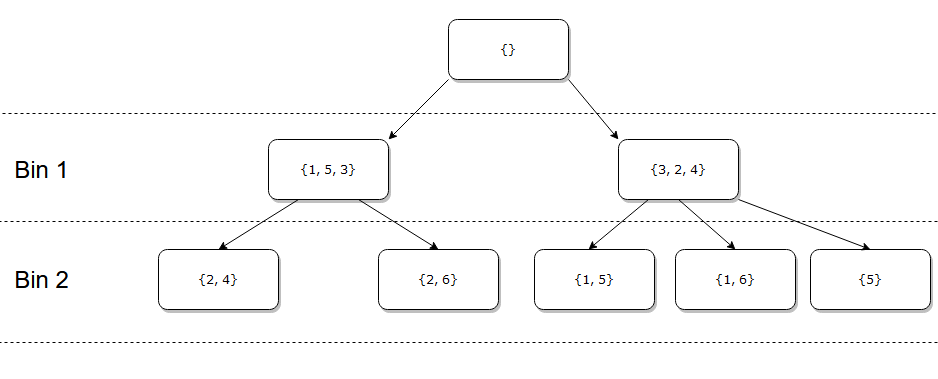
\includegraphics[width=0.9\textwidth]{bin_oriented.PNG}
\caption{Example of bin-based B\&B}
\end{figure}

A rationale for why this is a more efficient approach can be explained in terms of the depth and branching factors of the resulting trees.
In the item-based model, the depth of the tree is the number of items, while the branching factor at each depth is the number of feasible bins.
In contrast, the bin-based model makes the depth of the tree be the number of bins, while the branching factor at each depth is proportional to the amount of remaining items.
Since the number of leaves in a full tree is determined by $b^d$, where $b$ is the branching factor and $d$ is the depth,
having a higher depth is worse for performance than having a higher branching factor.

\subsection{Validating the Upper Bound}
The upper bound in multiple knapsack is calculated by combining the capacities of the remaining knapsacks into an aggregate knapsack and solving a single knapsack problem with the remaining items and this aggregate knapsack.
This reduced instance is often called the \emph{surrogate relaxed MKP} (SMKP).
The solution to the SMKP represents the best possible result we can expect from the current node, but there is no guarantee that a solution of that quality is feasible in our actual MKP.
\\ \\
Since the quality of this bound directly decides how much we are able to prune, having a bound that is too optimistic is of little help.
In an effort to lower this bound to something more realistic, many of the previous solutions to MKP, including MTM by Martello \& Troth \cite{martello_bound_1981} and Mulknap by Pisinger \cite{pisinger_exact_nodate},
introduce a way of validating that this upper bound is actually achievable. MTM was the first algorithm to introduce this notion, which is referred to as \emph{bound-and-bound}.
\\ \\
MTM does this by iteratively and greedily solving a series of single knapsack problems.
It essentially chooses a bin, fills it completely, reduces the instance by the bin and its items, picks a new bin and repeats until all the bins are filled, or we are out of items.
A different approach was implemented by Pisinger in his Mulknap algorithm.
Instead of solving multiple single knapsack problems, his approach relies on solving a subset sum problem for each bin while minimizing the remaining capacity of each bin.
If this results in assigning all the items to a bin, the upper bound has been validated.

\subsection{Path-symmetry}
Fukunaga introduces the concept of path-symmetry and a nogood in the article our work is based on \cite{fukunaga_branch-and-bound_2011}.
To understand path-symmetry, first we must introduce the notion of a nogood. Considering a node $N$ and its siblings $S_1 \ldots S_b$, we say that every sibling $S_i$ that has been expanded before N is a nogood with respect to each child, direct or indirect, of N.
In Figure \ref{fig:nogood}, S1 is a nogood with respect to C1 and C2 since S1 is a sibling of C1 and C2's parent N, and has already been expanded. Since bin-completion is a DFS-algorithm, every child of S1 has been exhaustively searched.
\\

\begin{figure}[h]
    \begin{center}
        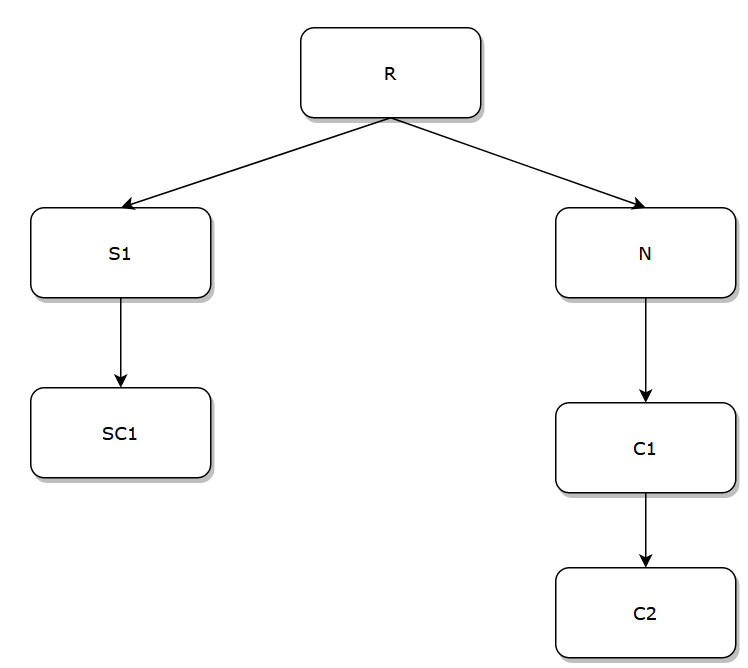
\includegraphics[width=0.5\textwidth]{nogood.PNG}
        \caption{Example of a nogood}
        \label{fig:nogood}
    \end{center}
\end{figure}

We define a path from some depth $d_1$ to $d_m$ as the union of the bins at each depth between $d_1$ and $d_m$.
For instance, the path from N ($d_1$) to C2 ($d_m$) is (N, C1, C2). The path items are the union of the items in each of these bins.

We say that there is path symmetry with respect to a nogood $S^{d_1}$ for some possible bin assignment $C^{d_m}$ and the path items $P$ from $d_1$ to $d_m$ given that:
\begin{enumerate}
    \item Every item in $S^{d_1}$ is in $P$.
    \item We can:
    \item[a)]Feasibly assign the items that are in $S^{d_1}$ to $N$
    \item[b)] Assign the remaining items in $(P \: \backslash \: N_{items})$ to the rest of the bins down to $d_m$ with all the assignments being feasible.
\end{enumerate}
If a path symmetry exists we can prune the node $C^{d_m}$, since it will achieve the same total value as the already expanded nogood.
b) is essentially an instance of the bin-packing problem, another NP-complete problem, but that can be approximately solved with a heuristic like first-fit-decreasing (FFD). 


\subsection{Maximin Share Fairness}


\section{Method and Implementation}
Here we will describe our experience with figuring out what to study, as well as how we went about implementing the algorithm.

\subsection{Inspiration}
The first step in this project was identifying what we wanted to study. Therefore, the start of the semester was largely spent familiarizing ourselves with the fair allocation field.
Initially, surveys such as ``Fair Division of Indivisible Goods: A Survey''\cite{amanatidis_fair_2022} were of great help in getting an overview of the field.
The open questions posed in that survey seemed somewhat daunting, and perhaps a bit more theoretical than we felt we had the capacity to contribute to.
\\ \\
However, applying different constraints seemed like a somewhat less developed part of the field, and was summarized nicely by Suksompong in 2021 \cite{suksompong_constraints_2021}.
Since the area of budget constraints had only really been studied by Wu et al \cite{wu_budget-feasible_2020}, it seemed like a natural and intriguing place to attempt to contribute.
Considering we wanted the project to involve the implementation of some algorithms, finding a fast way of solving budget constrained problem instances seemed like a good first step.
\\ \\
Due to the problem's similarity to the multiple knapsack problems, we started reviewing literature on ways of solving MKPs.
This work started with reading some of Kellerer et al's massive ``Knapsack problems'' book \cite{kellerer_knapsack_2004} and some of Pisinger's articles on the topic \cite{pisinger_exact_nodate}.
While they were helpful in understanding ways of solving the problem, the age of these algorithms (Pisinger's Mulknap-algorithm is from 1999) made us wonder if anything newer and better existed.
We then stumbled upon Fukunaga and Korf's bin-completion approaches \cite{fukunaga_bin_2007}, which were extended in Fukunaga's follow-up article in 2011 \cite{fukunaga_branch-and-bound_2011} with the notions of path dominance and path symmetry in order to prune even more of the state space.
The author's claims of outperforming the previous state of the art in low agent-to-item ratio instances and remaining competitive in high agent-to-item ratio problems made it an intriguing candidate.
\\ \\
Some further work was then done to ensure that there existed no solutions that were more recent and performed better. 
Specifically, we looked for later articles that referenced Fukunaga's work, but none seemed to present better alternatives.
We thereby concluded that Fukunaga's extended bin-completion algorithm from 2011 is the state of the art MKP-solver, and began our work with implementing it.

\subsection{Implementation}
Due to ease of use, speed, and familiarity among the supervisory team (including an existing library called Allocations.jl, which has been especially useful in understanding JuMP \cite{hetland_mlhetlandallocationsjl_nodate}), the implementations has been written in the Julia programming language.
Considering this was a new language for us, considerable time was spent in the beginning familiarizing ourselves with the language and its features. 
\\ \\
The implementation steps followed quite naturally from the pseudo-code presented in Fukunaga's article. 
Admittedly, there was a tendency in the beginning to go line for line, for instance attempting to read up on Pisinger's R2 reduction 
(which is not required for the algorithm to work, just an additional optimization step) before having a working solution.
After having learned this lesson in the early stages however, the focus quickly shifted to implementing the essentials and implementing what optimizations we had time for after that.
\\
\begin{algorithm}

    \centering
    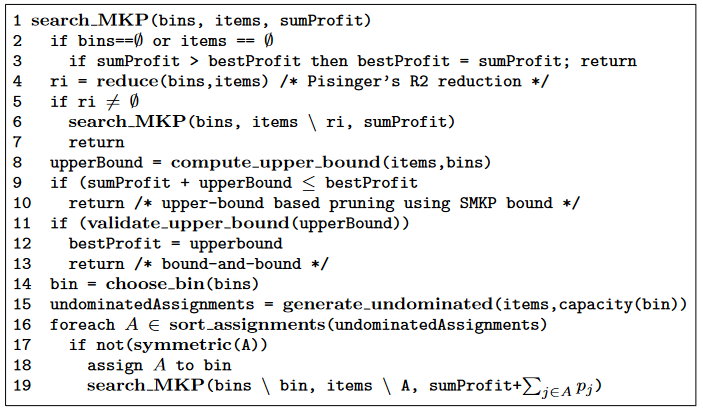
\includegraphics[width=1\textwidth]{psuedo_code.PNG}
    \caption{Pseudo-code for extended bin-completion \cite{fukunaga_branch-and-bound_2011}}

\end{algorithm}

The bare essentials of the algorithms are:

\begin{enumerate}
    \item Exit condition, line 2--3: If we're at a leaf node, check current profit against global maximum and update it if it is better.
    \item Upper bound, line 8--10: Compute the upper bound by combining the capacities of all remaining knapsacks and solving the single knapsack problem on the aggregate knapsack and the remaining items.
    If the profit so far plus this upper bound for the remaining subproblem is less than our global maximum, our current solution can not possibly be better than our best, so we prune.
    \item Choose bin, line 14: Decides which knapsack we should fill next. Chooses the knapsack with the least capacity among those that are not already filled.
    \item Undominated assignments, line 15: Generate all undominated, feasible and maximal assignments for the current bin.
    \item Fill bin and recurse, line 16 \& 18--19: Loop through all undominated assignments, sorted by cardinality with values as a tie-break, and solve each respective subproblem.
\end{enumerate}

In our current implementation, the above steps are those we have managed to implement, with a small caveat. 
The generation of undominated assignments is not yet finished, so the current version generates all combinations of the items,
and then checks if the assignment is feasible and maximal. This respectively ensures that the assignment fits in the knapsack, and no more items can fit in that assignment.
\\ \\
Our solution to the single knapsack problem relies on a dynamic programming approach to solve the problem in pesudo-polynomial time.
Since the only use of this algorithm is to calculate the upper bound, we can simply take the bottom right value of the resulting table and return it, 
while omitting the backtracking process. The actual steps in the solution don't matter, just the value it achieves. 
\\ \\
An additional feature not described in the pseudo-code is preprocessing of the items and knapsacks.
The implementation includes functions to remove items which are too large to fit into any knapsack and knapsacks which are too small to fit any items. 
\\ \\
After having implemented many of the above features, it seemed natural to produce something which we could compare out implementation to.
Seeing as we are yet to find the source code for the extended bin-completion algorithm, we had to think of alternative comparisons.
Linear programming approaches are a popular approach to solving similar problems, especially due to their ease of implementation.
We used the JuMP-library in Julia to implement the linear programming version, along with the CBC-optimizer \cite{dunning_jump_2017}.
At time of writing our code for the bin-completion algorithm is roughly 400 lines, while the equivalent JuMP-program is just 60 lines long.
Another advantage of the linear programming approach is that the program itself is written in a very similar way to the problem formulation, making it very readable.
For instance, comparing the initial formulation (\pageref{problem_formulation}) of the MKP in this article to the JuMP-program for solving the MKP (\pageref{alg:cap}), we can see that they are very reminiscent of each other.
\begin{algorithm}[H]
\caption{JuMP-program for MKP in Julia}\label{alg:cap}
\begin{algorithmic}
\State m = Model(Cbc.Optimizer) \Comment{Init model} 
\\
\State @variable(m, $x[1:n_{agents}, 1:n_{items}]$, binary = true) \Comment{Init binary variable}
\State @objective(m, Max, dot(values, x)) \Comment{Define objective}
\\
\For{\texttt{i in 1:$n_{agents}$}}\Comment{Ensure no bin exceeds its capacity}
    \State @constraint(m, dot($weights[i, :], x[i, :]$) $\leq$ capacities[i]) 
\EndFor
\\

\For{\texttt{i in 1:$n_{agents}$}} \Comment{Ensure no item is picked twice}
    \State@constraint(m, sum(x[:, i]) $\leq$ 1) 
\EndFor
\State optimize!(m) \Comment{Solve, please and thank you}
\end{algorithmic}
\end{algorithm}
    


\section{Experiments}
As sanity checks throughout the development of the algorithm, we utilized some examples of
multiple knapsack problems that we found online to make sure the algorithm was working correctly.
After having implemented working versions of both bin-completion and the JuMP-program we wrote code to pseudo-randomly generate problem instances.
These functions take as input the number of knapsacks/items, in addition to a range for values, weights and capacities.
The experiments conducted and presented in this article vary in number of agents and knapsacks, but have constant ranges for values, weights and capacities.
\\
These are:
\begin{enumerate}
    \item Values: 1--30
    \item Weights: 5--50
    \item Capacity: 30--120
\end{enumerate}
There is no real rationale behind these numbers beyond that they seemed somewhat reasonable.
In order to obtain a greater understanding of the algorithm's performance in different settings, this should be expanded upon in the follow-up project.
\\ \\
To ensure accurate measurements of performance, even on small instances, we used the ``BenchmarkTools.jl'' package to solve the instances several times, and return the mean time spent.
Perhaps in an effort to gild the lily, we run the benchmarking tool 3 times on each instance and record the mean of the means.
This procedure is then run on different instances with differing amounts of knapsacks and items to get wholistic understanding of the performance of the algorithms.
We tested this on 3 different algorithms. Our implementation of bin-completion (BC), our implementation without the preprocessing step of attempting to remove unfeasible bins and items (BC no pp),
and the JuMP-model with the CBC optimizer (JuMP - CBC).
\\ \\
Mostly to facilitate performance enhancement down the line, we also utilized the ``Profile'' and ``StatProfilerHTML.jl'' packages to
analyze where the majority of the runtime is spent, represented by a flame graph.
\subsection{Results}

\begin{figure}[H]
    \centering
    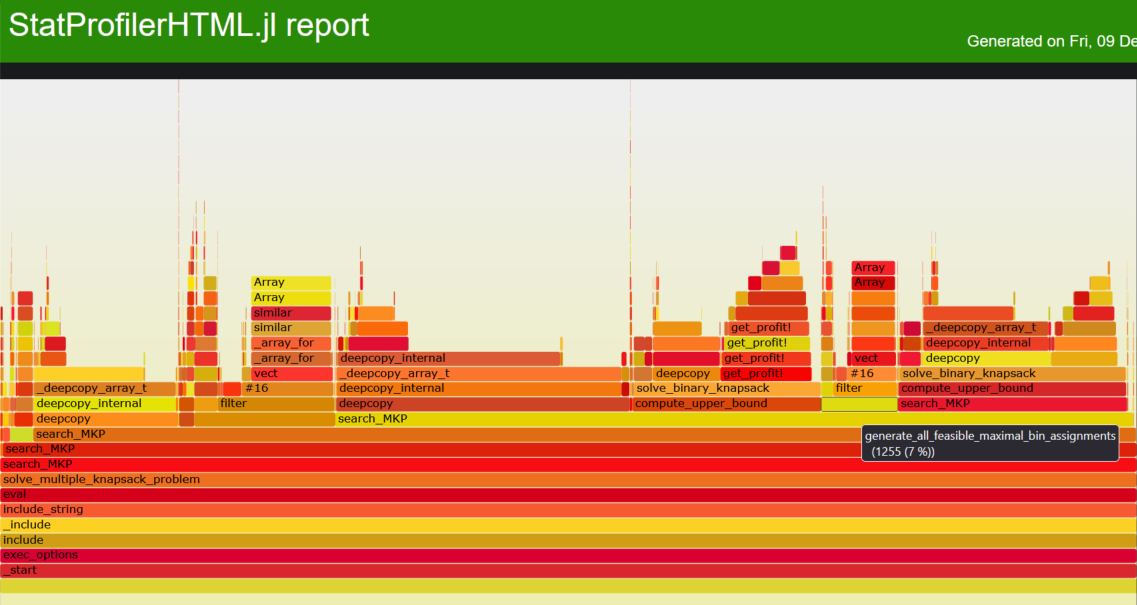
\includegraphics[width=1\textwidth]{flamegraph.PNG}
    \caption{Flame graph of our implementation of bin-completion}
\end{figure}
A flame graph works by taking samples of where execution is happening throughout the execution of a function.
The y-axis is essentially the depth of the call, with the top-level function call being at the bottom. Ignoring standard Julia calls, our top-level call is $solve\_multiple\_knapsack\_problem()$,
which then calls the recursive function $search\_MKP()$ to explore the tree.
The x-axis describes the proportion of time spent in different parts of the call.
We can for instance see that the $deepcopy()$ calls make up a significant proportion of the work being done. 

\begin{figure}[H]
    \centering
    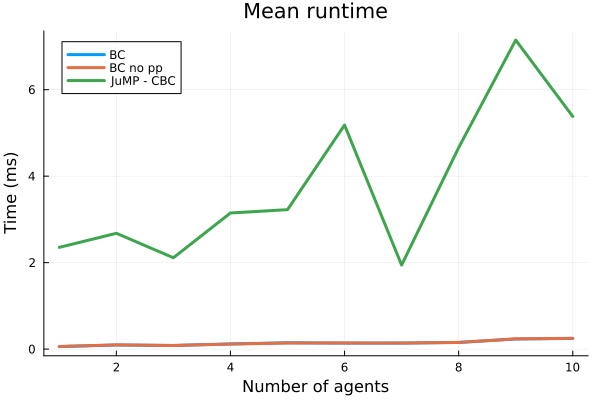
\includegraphics[width=0.8\textwidth]{mean_1-10agents_4items.png}
    \caption{The algorithms compared on instances with 4 items}
\end{figure}

\begin{figure}[H]
    \centering
    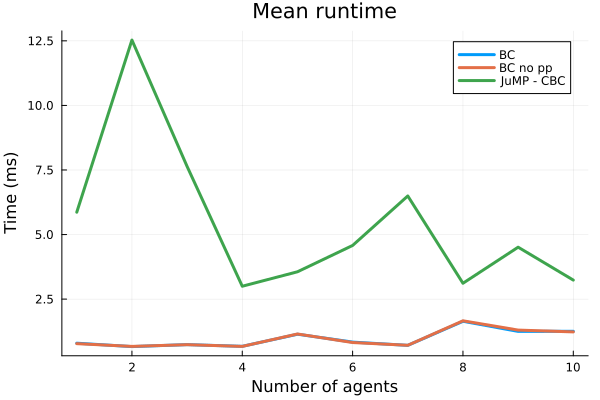
\includegraphics[width=0.8\textwidth]{mean_1-10agents_8items.png}
    \caption{The algorithms compared on instances with 8 items}
\end{figure}

\begin{figure}[H]
    \centering
    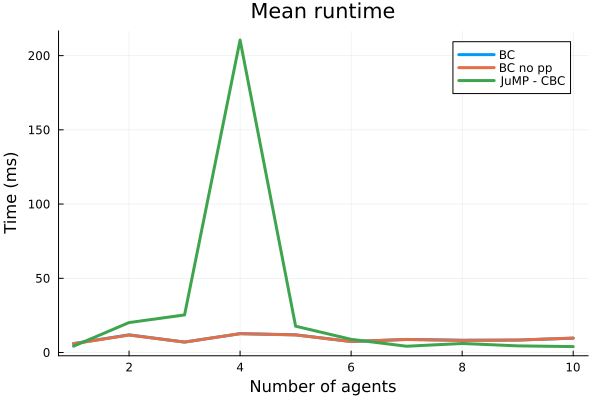
\includegraphics[width=0.8\textwidth]{mean_1-10agents_12items.png}
    \caption{The algorithms compared on instances with 12 items}
\end{figure}

\begin{figure}[H]
    \centering
    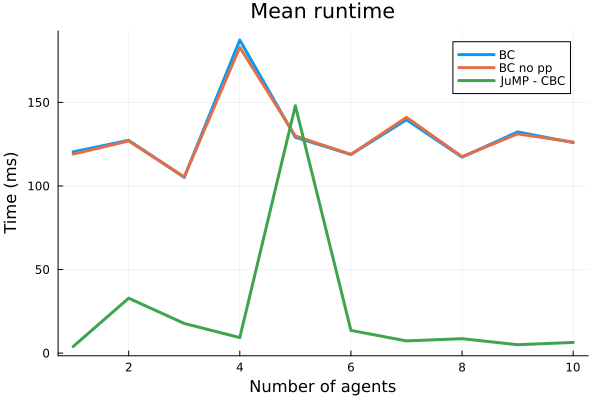
\includegraphics[width=0.8\textwidth]{mean_1-10agents_16items.png}
    \caption{The algorithms compared on instances with 16 items}
\end{figure}

\begin{figure}[H]
    \centering
    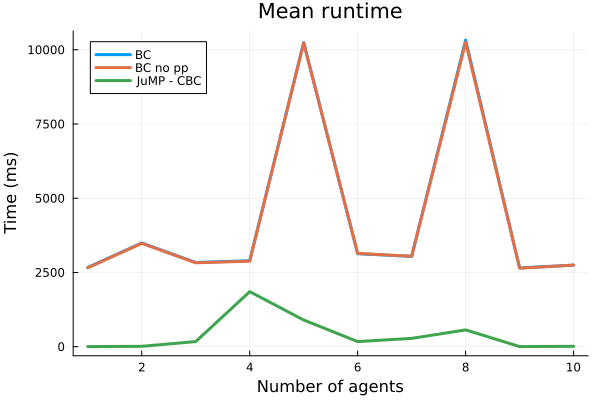
\includegraphics[width=0.8\textwidth]{mean_1-10agents_20items.png}
    \caption{The algorithms compared on instances with 20 items}
\end{figure} 

Notice that the scale of the y-axis changes between the plots.

\section{Discussion}
As expected, the runtime of the algorithms scales with the number of items.
In fact, there seems to be a relatively stable increase in the runtime of the bin-completion solution of around a factor of 10 for each 4 items added.
There does not seem to be any significant difference in the performance of our bin-completion implementation with and without preprocessing of the items.
While this \emph{could} be due to the preprocessing simply not being that useful, we are inclined to think that this is due to the parameters for the experiment.
In order for the preprocessing to remove an item, that item must be larger than the capacity of every knapsack in the instance, which is very unlikely in instances with weights between 5--50 and capacities between 30--120.
It becomes even less likely when the number of agents approaches 10, as it requires all 10 to have a capacity somewhere between 30--49, which only has odds of $\left(\frac{20}{90}\right)^{10}=\num[exponent-product = \cdot]{2.9e-7}$.
In addition, there would need to be an item of weight 50, which is also rather unlikely.
The odds of generating a knapsack with less capacity than the weight of all the items, such that it can be removed from the instance is also very unlikely under these parameters.
To be fair, the parameters of the experiment match a real world example relatively well, as the algorithm is unlikely to be asked to fit a fridge into one of several purses,
but expanding the range of the parameters would be interesting, such that we could see how the preprocessing step affects such scenarios.
\\ \\
An initially surprising discovery was that for instances with fixed amounts of items, e.g. 12, there doesn't seem to be much of an increase in the runtime with the number of agents.
Considering the number of knapsacks corresponds to the depth of the search tree, this was peculiar.
After some further analysis, it seems that the total weight of the items in the instances were too low.
Essentially, the 12 items would fit into for instance 4 knapsacks, making the algorithm terminate early, and never consider the additional knapsacks.
To be clear, this is a flaw of the experiment methodology, not the algorithm. It allocated all the items as it should, but got off the hook and didn't have to recurse as deeply is it could have. 
\\ \\
As for the performance of our bin-completion and the JuMP-model, the trend seems to be that there is some small static overhead in the JuMP-model which makes it slower in small instances.
Once the complexity of the instance goes up however, the JuMP-model seems to catch up to and surpass our current algorithm.
While this makes it look bleak for bin-completion, it's important to recall that our implementation is lacking in several areas.
Our implementation lacks Pisinger's R2 reduction, the validation of the upper bound (bound-and-bound) and the notion of path symmetry, all of which seem like worth wile pruning criteria.
\\ \\
The main take-away from the flame graph is that $deepcopy()$, which is called to ensure that changes to objects in the recursion don't affect the originals, is a very expensive operation.
Therefore, an investigation into whether every call is absolutely necessary, and if there are other, cheaper alternatives is warranted.
Somewhat surprisingly to us, generating every feasible and maximal allocation doesn't represent a very big proportion of the total runtime.
Still, it's significant enough to consider improving. Our implementation currently generates every combination of items and removes all which are non-feasible and non-maximal.
The assignment generation is bin-completion manages to directly generate all feasible assignments by traversing a binary tree, which would be a significant time save \cite{fukunaga_bin_2007}.
Another approach would be to greedily assign the lightest items until we fill the capacity of the bin, and generating all combinations up to k items, where k is the number of we filled we used to fill the bin.

\section{Conclusion}
We studied the leading bin-based algorithm for solving multiple knapsacks problems, bin-completion, and discussed ways in which it could be modified to be applicable to fair allocation problems with budget constraints.
The necessary extensions include allowing each agent to have different preferences for the items, and switching the focus from just maximizing value to introducing some fairness notion as a goal.
Specifically, the path-symmetry pruning criteria seems to inherently rely on identical valuations, which means it is not applicable to our planned algorithm for budget constrained fairness problems.
An implementation of parts of the bin-completion algorithm which lacks some pruning criteria was presented and evaluated against a similar linear programming solution.
We conclude that the current implementation is both harder to implement and struggles to compete with the performance of the linear program.
In addition, we discuss some possible problems with our experiments, namely that it only covers a narrow subset of possible problem instances. 
\\ \\
A quick analysis of the real runtime of the algorithm is presented in the form of a flame graph, and a discussion of possible improvements is presented.
These are namely preventing expensive copying operations and improving our generation of feasible assignments.
All in all, these results should not be taken to be any more than a comparison of the performance of a standard bin-based branch-and-bound algorithm to a linear problem.
The findings of Fukunaga with his bin-completion algorithm \cite{fukunaga_branch-and-bound_2011} seem very impressive in comparison,
but how many of the optimizations he presents still work, and how they perform with our planned extensions remains to be seen.

\section{Further Work}
\subsection{Our Scope}
In the second half of this project the goal will be to continue implementing the bin completion algorithm, as there are currently some missing parts.
The first step will be extending the algorithm to handle individual valuations, such that each agent can have their own preference for each item.
After this, a review of the currently missing pruning conditions: path-symmetry \cite{fukunaga_branch-and-bound_2011}, bound-and-bound \cite{martello_bound_1981} and Pisinger's R2 reduction
will be conducted in order to figure out which of them still work in the modified algorithm. The ones that do will then be implemented.
It currently seems to us that since path-symmetry relies on identical valuations to argue that there is a symmetry (i.e. that both paths will give the same total value), it will not be applicable to a setting with individual valuations.
Bound-and-bound to validate the upper bound seems to behave nicely with individual valuations, and \emph{``can be extremely powerful''} according to Fukunaga \cite{fukunaga_branch-and-bound_2011} 
It is therefore a major hope that this pruning criterion will translate well to our eventual algorithm, and offload some of the extra work that will be required to handle individual valuations.
Admittedly, we have not been able to identify which algorithm Fukunaga is referring to as ``Pisinger's R2 reduction'', and are therefore unsure of how important of an addition it is.
\\
In order to relate the problem to fair allocation, the algorithm will then be modified to maximize some other measure than total value.
The most obvious candidate is perhaps maximizing the product of the values, the maximum Nash welfare (MNW) solution, but seeing as this has already been studied by Wu et al \cite{wu_budget-feasible_2020},
other measures like egalitarian social welfare (ESW) or utilitarian social welfare (USW) may be more interesting to investigate.

\subsection{Interesting Follow-ups}
An interesting extension in addition to individual values would be individual weights. While the applications of this seem rather obscure to us currently,
this could for instance be useful in order to represent geometrically different knapsacks. Since disks more efficiently fill a cylinder than a square container,
perhaps this could have some uses for specific packing problems.
This extension seems to pose challenges for many of the pruning criteria discussed earlier, but perhaps there is some way to consolidate them.

\printbibliography[heading = bibintoc, title = References]

\end{document}